\documentclass[14pt,xcolor=pdftex,dvipsnames,table]{beamer}\usepackage[]{graphicx}\usepackage[]{color}
%% maxwidth is the original width if it is less than linewidth
%% otherwise use linewidth (to make sure the graphics do not exceed the margin)
\makeatletter
\def\maxwidth{ %
  \ifdim\Gin@nat@width>\linewidth
    \linewidth
  \else
    \Gin@nat@width
  \fi
}
\makeatother

\definecolor{fgcolor}{rgb}{0.345, 0.345, 0.345}
\newcommand{\hlnum}[1]{\textcolor[rgb]{0.686,0.059,0.569}{#1}}%
\newcommand{\hlstr}[1]{\textcolor[rgb]{0.192,0.494,0.8}{#1}}%
\newcommand{\hlcom}[1]{\textcolor[rgb]{0.678,0.584,0.686}{\textit{#1}}}%
\newcommand{\hlopt}[1]{\textcolor[rgb]{0,0,0}{#1}}%
\newcommand{\hlstd}[1]{\textcolor[rgb]{0.345,0.345,0.345}{#1}}%
\newcommand{\hlkwa}[1]{\textcolor[rgb]{0.161,0.373,0.58}{\textbf{#1}}}%
\newcommand{\hlkwb}[1]{\textcolor[rgb]{0.69,0.353,0.396}{#1}}%
\newcommand{\hlkwc}[1]{\textcolor[rgb]{0.333,0.667,0.333}{#1}}%
\newcommand{\hlkwd}[1]{\textcolor[rgb]{0.737,0.353,0.396}{\textbf{#1}}}%

\usepackage{framed}
\makeatletter
\newenvironment{kframe}{%
 \def\at@end@of@kframe{}%
 \ifinner\ifhmode%
  \def\at@end@of@kframe{\end{minipage}}%
  \begin{minipage}{\columnwidth}%
 \fi\fi%
 \def\FrameCommand##1{\hskip\@totalleftmargin \hskip-\fboxsep
 \colorbox{shadecolor}{##1}\hskip-\fboxsep
     % There is no \\@totalrightmargin, so:
     \hskip-\linewidth \hskip-\@totalleftmargin \hskip\columnwidth}%
 \MakeFramed {\advance\hsize-\width
   \@totalleftmargin\z@ \linewidth\hsize
   \@setminipage}}%
 {\par\unskip\endMakeFramed%
 \at@end@of@kframe}
\makeatother

\definecolor{shadecolor}{rgb}{.97, .97, .97}
\definecolor{messagecolor}{rgb}{0, 0, 0}
\definecolor{warningcolor}{rgb}{1, 0, 1}
\definecolor{errorcolor}{rgb}{1, 0, 0}
\newenvironment{knitrout}{}{} % an empty environment to be redefined in TeX

\usepackage{alltt}

% Specify theme
\usetheme{Madrid}
% See deic.uab.es/~iblanes/beamer_gallery/index_by_theme.html for other themes
\usepackage{caption}
\usepackage{tikz}
\usepackage{multirow}
% Specify base color
\usecolortheme[named=OliveGreen]{structure}
% See http://goo.gl/p0Phn for other colors

% Specify other colors and options as required
\setbeamercolor{alerted text}{fg=Maroon}
\setbeamertemplate{items}[square]

% Title and author information
\title{The Bond Market}
\author{Rob Hayward}
\IfFileExists{upquote.sty}{\usepackage{upquote}}{}
\begin{document}

\begin{frame}
\titlepage
\end{frame}


\begin{frame}{Outline}
\tableofcontents
\end{frame}


\section{Introduction}
\begin{frame}{Introduction}
\begin{itemize}
\item The bond market is the core of the capital markets
\item Government dominates the bond market due to high liquidity and low risk
\item Corporate bonds and LDC bonds offer higher return for a risk
\item Recent developments suggest reduced government liquidity
\item Quantitative easing 
\end{itemize}
\end{frame}



\section{Bond Calculation}
\begin{frame}{Bond price}
The value of the bond is just the discounted value of the payments that will be made
\begin{equation*}
P = \sum_{i = 1}^{i = n} \frac{C_i}{(1+r)^i} + \frac{M}{(1+r)^n}
\end{equation*}
Where $C$ is the coupon payment, $r$ is the rate at which future payments are discounted (the redemption yield), $M$ is the par value and $n$ is the number of years to maturity. 
\end{frame}

\section{Relative Value}
\begin{frame}{Relative Value}
A strategy that will assess the relative value of two bonds
\begin{itemize}
\item There is a standard relationship between yields
\item \textbf{Quantitative strategy} (return to normal)
\item \textbf{Fundamental strategy} (new relationship)
\end{itemize}
\end{frame}

\begin{frame}{German yield}
\begin{knitrout}
\definecolor{shadecolor}{rgb}{0.969, 0.969, 0.969}\color{fgcolor}

{\centering 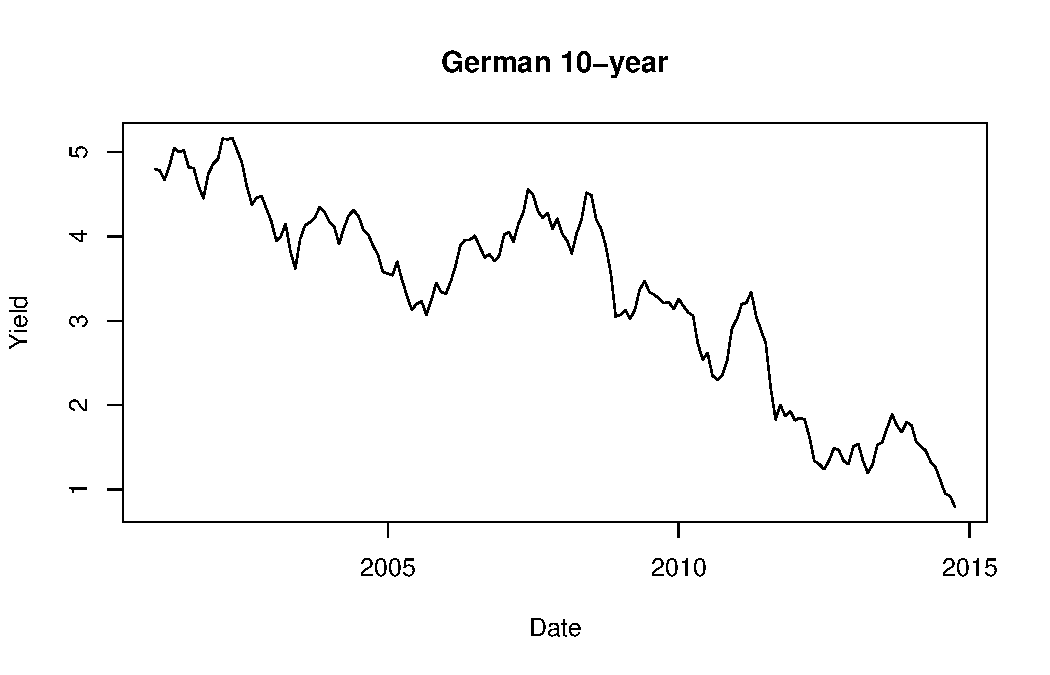
\includegraphics[width=\maxwidth]{figure/yield-1} 

}



\end{knitrout}
\end{frame}

\begin{frame}{Greek Risk Premium}
\begin{knitrout}
\definecolor{shadecolor}{rgb}{0.969, 0.969, 0.969}\color{fgcolor}

{\centering 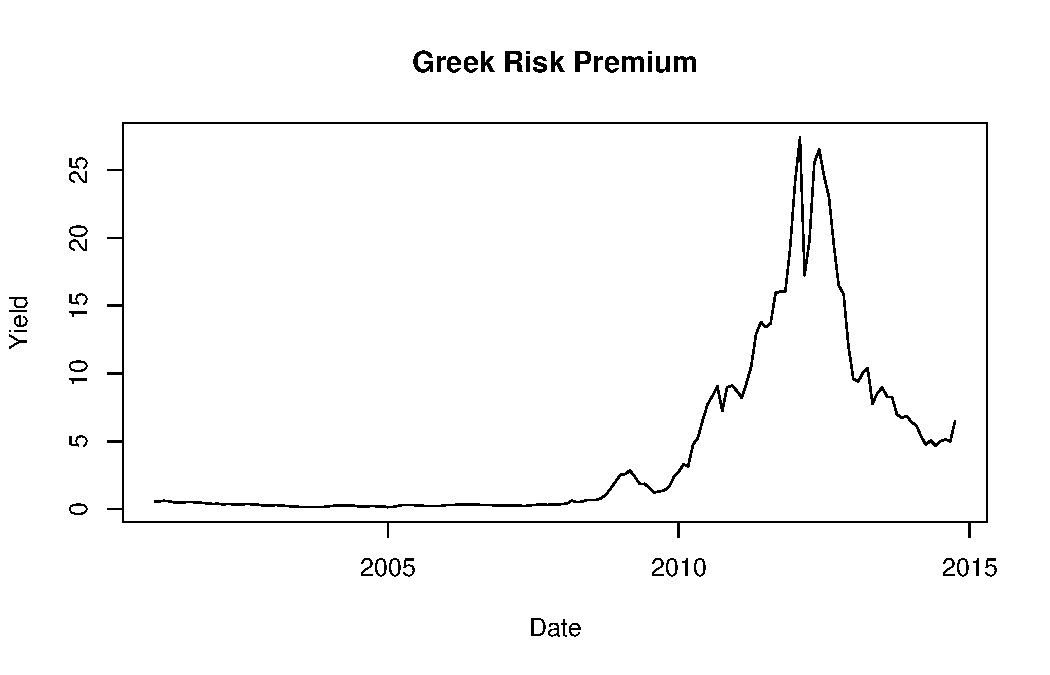
\includegraphics[width=\maxwidth]{figure/yield2-1} 

}



\end{knitrout}
\end{frame}

\begin{frame}{Italian Risk Premium}
\begin{knitrout}
\definecolor{shadecolor}{rgb}{0.969, 0.969, 0.969}\color{fgcolor}

{\centering 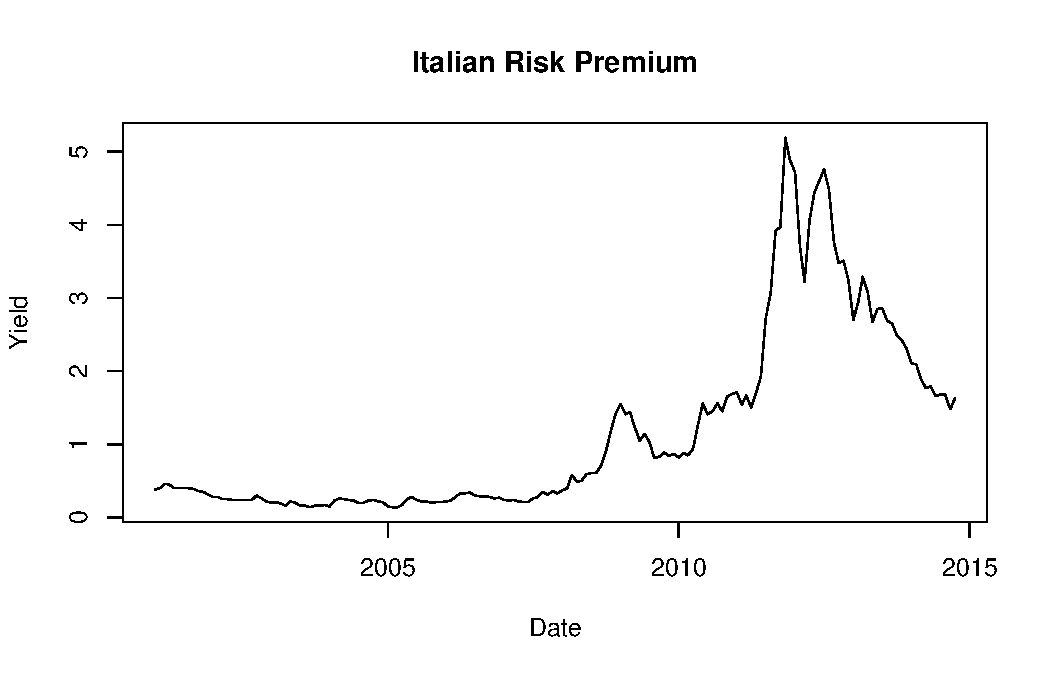
\includegraphics[width=\maxwidth]{figure/yield3-1} 

}



\end{knitrout}
\end{frame}


\section{Yield Curves}
\begin{frame}{Yield Curve Theory}
There are three main theories about the shape of the yield curve
\begin{itemize}
\item Expectations theory
\item Preferred habit or segmented market theory
\item Liquidity premium theory
\end{itemize}
\end{frame}

\begin{frame}{Expectations and Liquidity premium}
Expectations theory

\begin{itemize}
\item Return is $i^* = (1+i_i)(1+\hat{i}_2) -1$
\end{itemize}

if there  is a \emph{liquidity premium} $\theta_L = p(L)$

\begin{itemize}
\item Return is $i^* = (1+i_i)(1+\hat{i}_2) + \theta_L -1$ 
\end{itemize}

The liquidity premium is the balance between \emph{interest rate risk} and \emph{reinvestment risk}.

\end{frame}

\section{Credit}
\begin{frame}{Credit}
\begin{itemize}
\item The government curve provides the benchmark
\item Lower quality credit requires a \emph{risk premium} (denominated in bp)
\item Global and idiosyncratic factors will affect the risk premium
\end{itemize}
\end{frame}


\end{document}
